% LaTeX source for ``Algorithms for Computer Simulation of Molecular Systems''
% Copyright (c) 2023 รังสิมันต์ เกษแก้ว (Rangsiman Ketkaew).

% License: Creative Commons Attribution-NonCommercial-NoDerivatives 4.0 International (CC BY-NC-ND 4.0)
% https://creativecommons.org/licenses/by-nc-nd/4.0/

\chapter{กลศาสตร์ควอนตัมเชิงโมเลกุล}
\label{ch:mol_qm}

%----------------------------------------
\section{การจำลองเชิงตัวเลขและเทคนิคเชิงคอมพิวเตอร์}
%----------------------------------------

การจำลองเชิงตัวเลข (Numerical Modeling) คือวิธีที่การที่เราใช้ปัญหาทางคณิตศาสตร์และฟิสิกส์แบบต่าง ๆ เช่น นำมาใช้แก้สมการเชิง%
อนุพันธ์ที่ใช้ในการอธิบายปรากฏการณ์ต่าง ๆ ทางธรรมชาติซึ่งอาจจะมีความยากหรืออาจจะไม่มีทางแก้ได้ด้วยวิธีเชิงวิเคราะห์ (Analytical Method)
\idxboth{การจำลองเชิงตัวเลข}{Numerical Modeling}
\idxboth{วิธีเชิงวิเคราะห์}{Analytical Method}

สำหรับการจำลองด้วยเทคนิคเชิงคอมพิวเตอร์ (Computer Simulation) นั้นเป็นการศึกษาการตอบสนองเชิงพลวัต (Dynamic Response) 
ของระบบแบบจำลองต่อเงื่อนไขเริ่มต้น (Initial Conditions) ที่เราได้กำหนดไว้ โดยเงื่อนไขเริ่มต้นนี้สอดคล้องกับสภาวะจริงของระบบนั้น
\idxboth{เทคนิคเชิงคอมพิวเตอร์}{Computer Simulation}
\idxboth{เงื่อนไขเริ่มต้น}{Initial Conditions}

\begin{figure}[htbp]
    \centering
    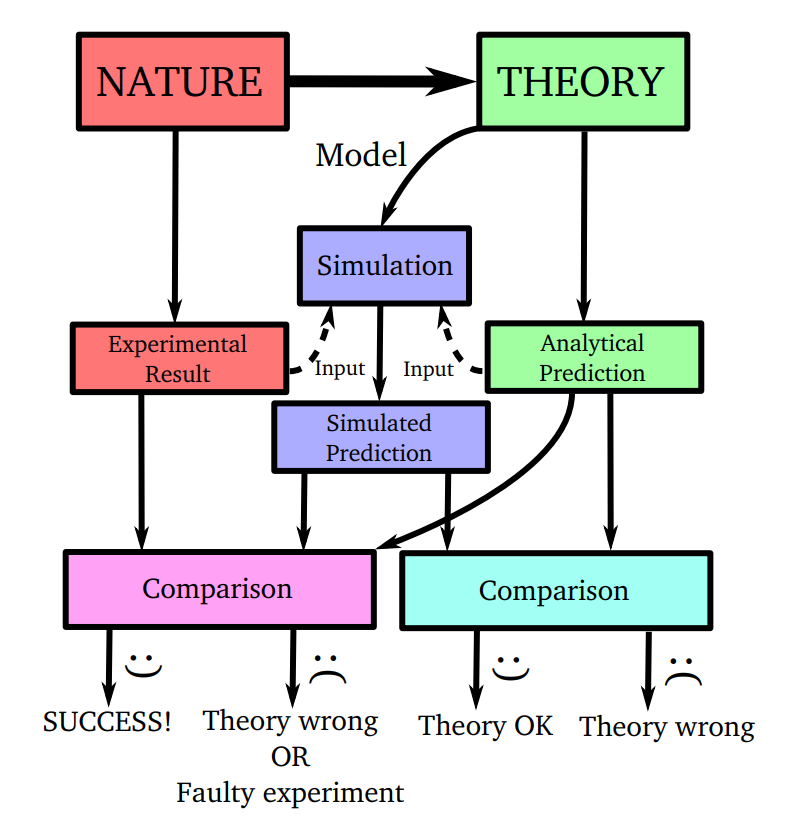
\includegraphics[width=0.8\linewidth]{fig/simulation-modeling-graph.png}
    \caption{แผนผังความเชื่อมโยงของระบบที่เราต้องศึกษา (Nature), ทฤษฎีหรือวิธีที่ใช้ในการศึกษา (Theory), แบบจำลองหรือโมเดล 
    (Model), ผลการทดลอง (Experimental Result), และผลการคำนวณหรือผลการทำนาย (Computational Results หรือ Prediction)}
    \label{fig:sim_model_graph}
\end{figure}

ภาพที่ \ref{fig:sim_model_graph} แสดงแผนผังเชื่อมโยงความแตกต่างระหว่าง Numerical Modeling กับ Computer Simulation 
นั้นก็คือใน Simulation นั้นระบบจำลองของเราจะถูกสร้างขึ้นมา เช่น เราสร้างระบบที่เป็นโมเลกุลน้ำหลาย ๆ โมเลกุลเกาะกลุ่มรวมกัน (Water 
Cluster) โดยเราหวังว่า Water Cluster ที่เราสร้างขึ้นมานี้จะสามารถเป็นตัวแทนของระบบของโมเลกุลน้ำจริง ๆ ได้ ซึ่งก็จะทำให้เราสามารถ%
ศึกษาคุณสมบัติต่าง ๆ ของโมเลกุลน้ำได้ตามต้องการ ส่วนการจำลองเชิงตัวหรือ Numerical Simulation นั้นจะเป็นการสร้างการทดลองเสมือนจริง 
(Virtual Experiments) ของระบบจำลองขึ้นมา อย่างไรก็ตามในบทความวิชาการทางด้านเคมีเชิงคำนวณหรือชีวเชิงคำนวณนั้นเรามักจะพบว่าคำว่า 
Modeling นั้นสามารถถูกแทนด้วยคำว่า Simulation ได้เช่นกัน

คำถามสำคัญที่หลายคนโดยเฉพาะอย่างนักวิทยาศาสตร์ที่ทำงานวิจัยเชิงการทดลองมักจะถามก็คือ \enquote{ทำไมการจำลองทางคอมพิวเตอร์ถึง%
มีความสำคัญ} คำตอบนั้นมีด้วยกันหลายข้อ ผู้เขียนขอสรุปเป็นประเด็นตามนี้ครับ

\begin{enumerate}
    \item การจำลองทางคอมพิวเตอร์นั้นเปรียบเสมือนเป็นสะพานเชื่อมโยงระหว่างทฤษฎีกับการทดลอง
    \item การทำการทดลองบางอย่างนั้นมีค่าใช้จ่ายที่สูงมากและมีความยากเพราะว่าตัวทฤษฎีนั้นซับซ้อนเกินไป ดังนั้นการจำลองทางคอมพิวเตอร์%
    นั้นจะเข้ามาช่วยในการจำลองการทดลองและทดสอบสมมติฐานเพื่อยืนยันทฤษฎีด้วย
    \item การจำลองทางคอมพิวเตอร์นั้นช่วยหาปัจจัยและเงื่อนไขที่เหมาะสมสำหรับการทดลองได้
    \item การจำลองทางคอมพิวเตอร์สามารถแสดงกระบวนการของระบบที่เราสนใจได้ ซึ่งอาจจะทำได้ยากในเชิงการทดลอง
    \item การจำลองทางคอมพิวเตอร์สามารถนำมาใช้ในการศึกษาปรากฏการณ์ที่การทดลองนั้นอาจจะให้ผลการทดลองที่ไม่ละเอียดพอ
\end{enumerate}

อย่างไรก็ตามผู้เขียนต้องขอสรุปเพิ่มเติมด้วยว่าการใช้แบบจำลองทางคอมพิวเตอร์เพียงอย่างเดียวนั้นจะเปล่าประโยชน์ถ้าหากว่าไม่มีผลการทดลองที่%
น่าเชื่อมายืนยันความถูกต้องของผลการคำนวณ ดังนั้นเคมีเชิงการทดลองกับเคมีเชิงคำนวณนั้นจึงเป็นศาสตร์ที่ต้องพึ่งพาอาศัยกัน

%----------------------------------------
\section{สมการชโรดิงเงอร์}
\idxboth{สมการชโรดิงเงอร์}{Schr\"{o}dinger Equation}
%----------------------------------------

สมการชโรดิงเงอร์เป็นสิ่งที่ช่วยให้เราสามารถเข้าใจพฤติกรรมของโมเลกุลได้ การที่เรารู้คำตอบหรือผลเฉลยของสมการนั้นนำไปสู่การเข้าใจข้อมูลต่าง ๆ
ของโมเลกุล (พูดให้ครอบคลุมกว่านี้คือระบบแบบ Microscopic) ที่อุณหภูมิ 0 K โดยสมการชโรดิงเงอร์ที่ขึ้นกับเวลา (Time-dependent 
Schr\"{o}dinger Equation) นั้นมีหน้าตาดังนี้

\begin{equation}
    \label{eq:time_dependent_schrodinger}
    \hat{\mathscr{H}} \Psi\left(\vec{r}_{1 \ldots N}, t\right) = 
    \mathrm{i} \hbar \frac{\partial \Psi\left(\vec{r}_{1 \ldots N}, t\right)}{\partial t}
\end{equation}

\noindent โดยที่ตัวแปรในสมการมีดังนี้
\begin{itemize}[topsep=0pt,noitemsep]
    \setlength\itemsep{1em}
    \item $\hat{\mathscr{H}}$ คือโอเปอร์เรเตอร์ของพลังงาน
    
    \item $\Psi$ คือฟังก์ชันคลื่นที่ขึ้นอยู่กับพิกัดหรือตำแหน่งของอนุภาค (ในที่นี้คืออิเล็กตรอน) ทั้งหมด $N$ ตัว เราจึงใช้เวกเตอร์แทน 
    $\vec{r}_{1}, \vec{r}_{2}, \dots, \vec{r}_{N}$ 
    
    \item $i$ คือหน่วยจินตภาพ $(\sqrt{-1})$
    
    \item $\hbar$ คือค่าคงที่ของพลังค์แบบลดรูป (Reduced Planck's constant) มีค่าเท่ากับ 
    \num{1.05457182e-34} \unit{m^{2}.kg.s^{-1}}
\end{itemize}

ตัวแปรที่น่าจะมีความสำคัญที่สุดก็คือ $\hat{H}$ ซึ่งเป็นโอเปอร์เรเตอร์ที่ที่เป็นผลรวมของโอเปอร์เรเตอร์พลังงานศักย์และโอเปอร์เรเตอร์พลังงานจลน์ 
ดังนี้

\begin{equation}
    \label{eq:hamiltonian_operator}
    \hat{\mathscr{H}}=\hat{\mathscr{T}}+\hat{V}
\end{equation}

\noindent โดยที่โอเปอร์เรเตอร์พลังงานจลน์ของระบบ $\hat{\mathscr{T}}$ นั้นก็คือผลรวมของโอเปอร์เรเตอร์พลังงานจลน์ของอนุภาคแต่ละตัวนั่นเอง

\begin{equation}
    \label{eq:kinetic_operator}
    \hat{\mathscr{T}}=\sum_{i=1}^N \frac{-\hbar^2}{2 m_i} \nabla_i^2
\end{equation}

\noindent โดยที่ $m_i$ คือมวลของอนุภาค $i$, $N$ คือจำนวนของอนุภาค และ $\nabla_i^2$ คือ Laplacian ในพิกัดคาร์ทีเซียนของอนุภาค 
$i$ ซึ่งมีสมการดังนี้

\begin{equation}
    \label{eq:nabla}
    \nabla_i^2=\frac{\partial^2}{\partial x_i^2}+\frac{\partial^2}{\partial y_i^2}+\frac{\partial^2}{\partial z_i^2}
\end{equation}

\noindent โดยที่ $\vec{r}_i=\left(x_i, y_i, z_i\right)$ คือเวกเตอร์ของตำแหน่งในพิกัดคาร์ทีเซียน 

ส่วนพลังงานจลน์ของระบบ ($\hat{V}\left(\vec{r}_{1 \ldots N}\right)$) นั้นจริง ๆ แล้วมีความซับซ้อนมากเพราะว่าประกอบไปด้วย%
พลังงานจลน์หลาย ๆ รูปแบบมารวมกันแล้วก็จะมีความเฉพาะต่อระบบที่เราศึกษา สำหรับเคมีนั้นระบบที่เราสนใจศึกษาคือโมเลกุลดังนั้นโอเปอร์เรเตอร์%
พลังงานศักย์นั้นจะต้องสอดคล้องกับพลังงานศักย์ของนิวเคลียสและอิเล็กตรอนเป็นหลักซึ่งผู้อ่านจะได้ศึกษาในหัวข้อที่ 

คราวนี้เรากลับมาดูที่ฟังก์ชันคลื่นกันต่อ ถ้าหากว่าฟังก์ชันคลื่นของเรานั้นเป็นฟังก์ชันที่ขึ้นอยู่กับตำแหน่งของอนุภาคเพียงอย่างเดียวและไม่ขึ้นกับเวลา 
เราสามารถเขียนฟังก์ชันคลื่นของทั้งระบบให้อยู่ในรูปผลคูณของฟังก์ชันคลื่นของอนุภาคแต่ละตัวได้โดยใช้เทคนิคที่เรียกว่า Separation of Variables 
ซึ่งเราจะได้สมการดังนี้

\begin{equation}
    \Psi\left(\vec{r}_{1 \ldots N}, t\right)=\psi\left(\vec{r}_{1 \ldots N}\right) \theta(t)
\end{equation}

\noindent ซึ่งเมื่อเรานำสมการด้านบนแทนเข้าไปในสมการชโรดิงเงอร์เราจะได้สมการดังนี้

\begin{equation}
    \frac{1}{\psi} \hat{H} \psi=\mathrm{i} \hbar \frac{1}{\theta} \frac{\partial \theta}{\partial t}
\end{equation}

เนื่องจากว่าฝั่งซ้ายของสมการนั้นเป็นฟังก์ชันที่ขึ้นกับ $\vec{r}_{1 . . . N}$ อย่างเดียวและฝั่งขวานั้นเป็นฟังก์ชันที่ขึ้นกับ $t$ ดังนั้นทั้งสองฝั่ง%
นั้นจะต้องมีค่าเท่ากับค่าคงที่ค่าหนึ่งซึ่งก็คือพลังานของระบบ $E$ แล้วเราจะได้ว่าสมการโชรดิงเงอร์ที่ขึ้นกับเวลานั้นจะเปลี่ยนเป็นสมการชโรดิงเงอร์ที่%
ไม่ขึ้นกับเวลา (Time-independent Schr\"{o}dinger Equation) ซึ่งมีสมการดังนี้

\begin{equation}
    \label{eq:time_independent_schrodinger}
    \hat{\mathscr{H}} \psi=E \psi
\end{equation}

สำหรับ Hamiltonians เกือบทั้งหมด (ไม่ใช้ทุกอัน) นั้นจะมีผลเฉลยสำหรับ Time-independent Schr\"{o}dinger Equation ที่มีค่าที่แน่นอน 
(Quantized) สำหรับแต่ละ State $n$ ของอนุภาค ดังนี้

\begin{equation}
    \hat{\mathscr{H}} \psi_n=E_n \psi_n
\end{equation}

\noindent ซึ่งเราสามารถตีความสมการด้านบนได้ว่าอนุภาคควอนตัมที่อยู่ในสถานะที่ $n$ จะมีค่าพลังงานที่แน่นอนนั้น $E_n$ นอกจากนี้แล้วสมการ%
ด้านบนนั้นเป็นปัญหาแบบค่าไอเกน (Eigenvalue Problem) โดยที่ $E_n$ คือค่าไอเกนและ $\psi_n$ คือฟังก์ชันไอเกนของโอเปอร์เรเตอร์ 
$\hat{\mathscr{H}}$ ซึ่งการที่เราจะแก้สมการ Time-independent Schr\"{o}dinger Equation นั้นจะต้องอาศัยเทคนิคพิเศษซึ่งจะได้ศึกษา%
ต่อในบทต่อ ๆ ไป\footnotetext{ตั้งแต่ส่วนนี้ของหนังสือเป็นต้นไปสมการโชรดิงเงอร์ (Schr\"{o}dinger Equation) นั้นจะหมายถึงสมการ%
ชโรดิงเงอร์แบบที่ไม่ขึ้นกับเวลา (Time-independent Schr\"{o}dinger Equation) ถ้าหากผู้เขียนต้องการที่จะใช้คำว่าสมการชโรดิงเงอร์แบบ%
ที่ขึ้นกับเวลา (Time-dependent Schr\"{o}dinger Equation) ก็จะเขียนใช้คำนี้ตรง ๆ เลย}

%----------------------------------------
\section{แฮมิลโทเนียนเชิงโมเลกุล}
\idxboth{แฮมิลโทเนียนเชิงโมเลกุล}{Hamiltonian!Molecular Hamiltonian}
%----------------------------------------

ในวิชาเคมีควอนตัมนั้นเราจะนิยามว่าโมเลกุลนั้นประกอบไปด้วยอิเล็กตรอน $n$ ตัวและนิวเคลียส $N$ ตัว โดยมีคุณสมบัติดังต่อไปนี้

\begin{itemize}[topsep=0pt,noitemsep]
    \setlength\itemsep{1em}
    \item อิเล็กตรอนมีประจุเท่ากับ $-e$ 
    \item อิเล็กตรอนมีมวลเท่ากับ $m_e$ 
    \item นิวเคลียสตัวที่ $I$ นั้นมีประจุเท่ากับ $Z_I e$ 
    \item นิวเคลียสตัวที่ $I$ มีมวลเท่ากับ $m_I$ 
\end{itemize}

\noindent โดยที่อิเล็กตรอนกับนิวเคลียสนั้นจะถูกพิจารณาว่าเป็นจุดประจุ (Point Charges) 

โอเปอร์เรเตอร์พลังงานจลน์ $\hat{\mathscr{T}}$ สำหรับโมเลกุลนั้นเราสามารถประยุกต์ใช้สมการที่ \ref{eq:kinetic_operator} ได้ซึ่งก็%
คือพลังงานจลน์ของทั้งอิเล็กตรอนและนิวเคลียสรวมกัน ดังนี้

\begin{equation}
    \label{eq:kinetic_operator_molecule}
    \hat{\mathscr{T}} = \underbrace{\sum_{I=1}^N \frac{-\hbar^2}{2 m_I} \nabla_I^2}_{\text {nuclei }} 
    + \underbrace{\sum_{i=1}^n \frac{-\hbar^2}{2 m_e} \nabla_i^2}_{\text {electrons }}
\end{equation}

ส่วนโอเปอร์เรเตอร์พลังงานศักย์ $\hat{V}$ สำหรับโมเลกุลนั้นก็จะเป็นอันตรกิริยาคูลอมป์ (Coulomb Interaction) ระหว่างจุดประจุ ดังนี้

\begin{equation}
    \label{eq:potential_operator_molecule}
    \hat{\mathcal{V}} = 
    \underbrace{\sum_{\substack{I=1,1}}^N \frac{Z_I Z_J e^2}{4 \pi \varepsilon_0 R_{I J}}}_{\text{nucleus-nucleus}}
    + \underbrace{\sum_{i=1}^n \sum_{I=1}^N \frac{-Z_I e^2}{4 \pi \varepsilon_0 r_{i I}}}_{\text{electron-nucleus}}
    + \underbrace{\sum_{\substack{i=1,1 \\ j=i+1}}^n \frac{e^2}{4 \pi \varepsilon_0 r_{i j}}}_{\text{electron-electron}},
\end{equation}

\noindent ซึ่งก็คืออันตรกิริยาระหว่างทุกคู่ที่เป็นไปได้ นั่นคือ Nucleus-Nucleus, Electron-Nucleus และ Electron-Electron 
ส่วน $Z_I e$ นั้นก็คือประจุของนิวเคลียสที่ $I$ ซึ่ง $Z_I$ นั้นก็คือเลขอะตอมของนิวเคลียส เช่น ไฮโดรเจนนั้นก็จะมี $Z_I = 1$ และคาร์บอน%
ก็จะมี $Z_I=6$ ส่วน $e$ นั้นคือประจุของอิเล็กตรอนซึ่งก็คือ $-e$ นั่นเอง 

โดยปกติแล้วเรามักจะใช้ตัวห้อยที่เป็นอักษรภาษาอังกฤษตัวใหญ่ $I, J, K, \ldots$ เพื่อบ่งบอกถึงนิวเคลียสและใช้ตัวอักษรตัวเล็กสำหรับอิเล็กตรอน  
แล้วก็จะใช้ $R$ แทนระยะห่างที่วัดจากนิวเคลียสและใช้ $r$ แทนระยะห่างที่วัดจากอิเล็กตรอนอย่างน้อยหนึ่งตัว อย่างไรก็ตามในเคมีควอนตัมนั้นเรา%
มักจะใช้หน่วยของปริมาณต่าง ๆ ในหน่วยอะตอม (atomic units หรือ a.u.) แทนที่จะใช้หน่วย SI เพราะว่าสะดวกต่อการคำนวณโดยสามารถดู%
ได้ตามตาราง 

\begin{equation*}
    \begin{array}{|l|ll|}
        \hline \text {Charge of electron: } e=-1 & \text {Length: } & 1 \mathrm{bohr} = 0.529177 \AA \\
        \text {Mass of electron: } m_e=1 & \text {Energy: } & 1 \text { hartree } = 2625.4996 \mathrm{~kJ} / \mathrm{mol} \\
        \hbar=h / 2 \pi=1 & & 1 \text { hartree } = 27.2113845 \mathrm{eV} \\
        4 \pi \varepsilon_0=1 & & \\
        \hline
    \end{array}
\end{equation*}

ถ้าเราเขียนโอเปอร์เรเตอร์พลังงานจลน์โดยใช้ atomic units จะได้ดังนี้

\begin{equation}
    \label{eq:kinetic_operator_au}
    \hat{\mathscr{T}} = \underbrace{-\frac{1}{2} \sum_{I=1}^N \frac{1}{m_I} \nabla_I^2}_{\text{nuclei}} 
    - \underbrace{\frac{1}{2} \sum_{i=1}^n \nabla_i^2}_{\text {electrons }},
\end{equation}

\noindent และสำหรับโอเปอร์เรเตอร์พลังงานศักย์

\begin{equation}
    \label{eq:potential_operator_au}
    \hat{V} = \underbrace{\sum_{\substack{I=1, J=I+1}}^N \frac{Z_I Z_J}{R_I}}_{\text{nucleus-nucleus}} 
    + \underbrace{\sum_{i=1}^n \sum_{I=1}^N \frac{-Z_I}{r_{i I}}}_{\text{electron-nucleus}} 
    + \underbrace{\sum_{\substack{i=1,1 \\ j=i+1}}^n \frac{1}{r_{i j}}}_{\text{electron-electron}} .
\end{equation}

\noindent ซึ่งถ้าหากเราเขียน Hamiltonian ของโมเลกุล $\hat{\mathscr{H}}^{\mathrm{mol}}$ โดยรวมโอเปอร์เรเตอร์ทั้งสองตัวเข้าด้วยกัน 
จะได้ดังนี้

\begin{equation}
    \label{eq:hamiltonian_operator_molecule}
    \hat{\mathscr{H}}^{\mathrm{mol}}=\hat{\mathscr{T}}_n+\hat{\mathscr{T}}_e+\hat{V}_{n n}+\hat{V}_{e n}+\hat{V}_{e e}
\end{equation}

\noindent โดยสองเทอมแรกนั้นก็คือพลังงานจลน์และสามเทอมที่เหลือนั้นก็คือพลังงานศักย์คูลอมป์

%----------------------------------------
\section{คุณสมบัติพื้นฐานของฟังก์ชันคลื่น}
%----------------------------------------

โอเครครับ เราได้ศึกษาโอเปอร์เรเตอร์ Hamiltonian กันไปคร่าว ๆ แล้ว ในหัวข้อนี้เราจะมาดูรายละเอียดของฟังก์ชันคลื่นกันซึ่งผู้เขียนจะขออธิบาย%
คุณสมบัติพื้นฐานของฟังก์ชันคลื่นก่อนซึ่งถือว่าเป็นพื้นฐานสำคัญมาก ๆ ที่ผู้อ่านควรจะต้องทราบและเข้าใจก่อนที่จะไปศึกษาฟังก์ชันคลื่นแบบเชิงลึกต่อ%
ไปในบทอื่น ๆ โดยคุณสมบัติของฟังก์ชันคลื่นที่ผู้เขียนเลือกมาอธิบายนั้นจะเป็นคุณสมบัติที่สำคัญ ๆ เท่านั้นซึ่งจำเป็นและเพียงพ่อต่อการทำความเข้าใจ%
ในบทต่อ ๆ ไป

ก่อนอื่นเลยผู้เขียนขออ้างการตีความฟังก์ชันคลื่นของบอนส์ (Born's Interpretation) ที่ว่า $\psi_i^* \psi_i \mathrm{~d} \tau$ 
นั้นคือความน่าจะเป็นสำหรับอนุภาคที่อยู่ในสภาวะ $i$ ในอนุภาคที่มีปริมาตรเล็กมาก ๆ ($\mathrm{d} \tau$) โดยที่ $\psi_i^*$ นั้นแทน%
คอนจูเกตเชิงซ้อน (Complex Conjugate) ของฟังก์ชันคลื่น $\psi_i$ นั่นหมายความว่าฟังก์ชันคลื่นอาจจะมีส่วนเชิงซ้อนเป็นองค์ประกอบก็ได้ 
อย่างไรก็ตามความน่าจะเป็น $\psi_i^* \psi_i \mathrm{~d} \tau$ มีเฉพาะส่วนจริงเป็นองค์ประกอบเท่านั้นซึ่งสอดคล้องกับเงื่อนไขที่ว่า%
จะต้องสามารถสังเกตได้ (Observable) 

กำหนดให้ความน่าจะเป็นสำหรับสถานะที่ $i$ ซึ่งเขียนแทนด้วย $\rho_i(\vec{r})$ นั้นถูกทำให้เป็นปกติ (ถูก Normalized แล้ว) เราจะตีความ%
ได้ว่าความน่าจะเป็นรวมที่จะพบอนุภาคที่ตำแหน่งไหนก็ตามใน Space นั้นจะมีค่าเท่ากับ 1 ซึ่งเขียนแทนด้วยสมการดังนี้

\begin{equation}
    \int_{\text{all space}} \rho_i \mathrm{~d} \tau=\int_{\text {all space }} \psi_i^* \psi_i \mathrm{~d} \tau=1,
\end{equation}

\noindent โดยที่ $\mathrm{d} \tau$ คือปริมาตรในพิกัดคาร์ทีเซียนสำหรับอนุภาคหนึ่งตัวซึ่งมีนิยามแบ่งตามพิกัดอ้างอิง ดังนี้

\begin{itemize}
    \item พิกัดคาร์ทีเซียน $\mathrm{d} \tau=\mathrm{d} x \mathrm{~d} y \mathrm{~d} z$ 
    
    \item พิกัดเชิงขั่วมีนิยามคือ $\mathrm{d} \tau=r^2 \sin (\theta) \mathrm{d} r \mathrm{~d} \theta \mathrm{d} \varphi$
\end{itemize}

\noindent ซึ่งถ้าหากเราทำอินทิเกรตทั่วทั้งปริมาตรเราสามารถละขอบเขตการอินทิเกรตออกไปได้ ดังนี้

\begin{equation}
    \int_{\text{all space}} \ldots \mathrm{d} \tau \equiv \int \ldots \mathrm{d} \tau \text {. }
\end{equation}

นอกจากนี้เรายังพบว่าถ้า $\psi$ นั้นถูก Normalized แล้ว $\Psi(t)$ ก็จะถูก Normalized ด้วย ซึ่งเราก็จะได้ความสัมพันธ์ดังนี้ 

\begin{equation}
    \Psi^*(t) \Psi(t)=\psi^* \psi
\end{equation}

สำหรับนิยามถัดมาก็คือโอเปอร์เรเตอร์ $\hat{\Omega}$ ซึ่งมีค่าคาดหวัง (Expectation Value) สำหรับระบบในสถานะ $i$ 
$(\langle\Omega\rangle_i)$ ดังนี้

\begin{equation}
    \langle\Omega\rangle_i \equiv 
    \frac{\int \psi_i^* \hat{\Omega}_i \psi_i \mathrm{~d} \tau}{\int \psi_i^* \psi_i \mathrm{~d} \tau}
\end{equation}

\noindent สำหรับฟังก์ชันคลื่นที่ถูก Normalized แล้วนั้น $(\langle\Omega\rangle_i)$ จะกลายเป็น

\begin{equation}
    \langle\Omega\rangle_i=\int \psi_i^* \hat{\Omega}_i \mathrm{~d} \tau
\end{equation}

แล้วก็ถ้าหากว่า $\psi_i$ เป็นฟังก์ชันไอเกนของ $\hat{\Omega}$ เราจะได้ว่า

\begin{equation}
    \langle\Omega\rangle_i 
    = \frac{\int \psi_i^* \hat{\Omega} \psi_i \mathrm{~d} \tau}{\int \psi_i^* \psi_i \mathrm{~d} \tau} 
    = \frac{\Omega_i \int \psi_i^* \psi_i \mathrm{~d} \tau}{\int \psi_i^* \psi_i \mathrm{~d} \tau} 
    = \Omega_i
\end{equation}

\noindent นั่นหมายความว่า Expectation Value นั้นมีค่าเท่ากับค่าไอเกน (Eigenvalue) หรือ $\Omega_i$ นั่นเอง ดังนั้นเราจึงสามารถ%
เขียนนิยามของพลังงานของระบบในสถานะ $i$ $(E_i)$ ในรูปของ Expectation Value ของ Hamiltonian สำหรับฟังก์ชันคลื่นที่ถูก 
Normalized แล้วได้ดังนี้ 

\begin{equation}
    E_i = \int \psi_i^* \hat{\mathcal{H}} \psi_i \mathrm{~d} \tau
\end{equation}

อย่างไรก็ตามในการพิสูจน์สมการต่าง ๆ ในกลศาสตร์ควอนตัมนั้นถ้าหากว่าเราต้องมาเขียนนิยามของพลังงานหรือพารามิเตอร์อื่น ๆ โดยใช้สมการ%
คณิตศาสตร์ตามด้านบนนั้นก็จะมีความยุ่งยากและเสียเวลา ดังนั้นเพื่อเป็นการทำให้การเขียนนิยามต่าง ๆ นั้นง่ายและกระชับขึ้น Paul Dirac จึงได้%
เสนอให้ใช้สัญกรณ์ที่เรียกว่า Dirac bra-c-ket Notation ดังนี้

\begin{equation}
    \left\langle\psi_i|\hat{\Omega}| \psi_j\right\rangle 
    \equiv \langle i|\hat{\Omega}| j\rangle 
    \equiv \int \psi_i^* \hat{\Omega}_j \mathrm{~d} \tau
\end{equation}

\noindent โดยที่ $\left\langle\psi_i\right|$ หรือ $\langle i|$ นั้นเรียกว่า bra ของฟังก์ชันคลื่นของสถานะที่ $i$ และอีกตัวก็คือ 
$\left|\psi^j j\right\rangle$ หรือ $|j\rangle$ นั้นเรียกว่า ket ซึ่งใช้แทนฟังก์ชันคลื่นของสถานะที่ $j$

เนื่องจากว่า Hamiltonian ของโมเลกุลนั้นมีคุณสมบัติที่เป็นเมทริกซ์แบบ Hermitian ดังนั้นเราจึงสามารถใช้คุณสมบัติการเปลี่ยนรูปดังต่อไปนี้ได้

\begin{equation}
    \int \psi_i^* \hat{\Omega} \psi_j \mathrm{~d} \tau 
    = \int\left(\hat{\Omega} \psi_i\right)^* \psi_j \mathrm{~d} \tau
\end{equation}

\noindent ซึ่งเราพบว่าค่าไอเกนของมันนั้นเป็นส่วนจริงเท่านั้นและฟังก์ชันไอเกนนั้นเป็น Orthogonal นอกจากนี้ถ้าหากเรามาดูที่พลังงานของระบบ%
เราจะพบว่าพลังงานนั้นเป็นปริมาณที่สามารถวัดค่าได้ ดังนั้นพลังงานนั้นจะต้องเป็นค่าจริง (Real) เสมอ ดังนั้นจึงเป็นการยืนยันได้อีกว่า Hamiltonian 
นั้นจะต้องเป็น Hermitian 

สำหรับ Orthonormal States (สถานะของฟังก์ชันคลื่นที่เป็นทั้ง Orthogonal และ Normalized)

\begin{equation}
    \int \psi_i^* \psi_j \mathrm{~d} \tau 
    \equiv \left\langle\psi_i \mid \psi_j\right\rangle 
    \equiv \langle i \mid j\rangle=\delta_{i j}
\end{equation}

\noindent โดยที่ $\delta_{i j}$ นั้นคือ Kroenecker Delta Function ซึ่งจะมีค่าเท่ากับ 1 เมื่อ $i=j$ และเท่ากับ 0 เมื่อ $i \neq j$

ถ้าผู้อ่านต้องการศึกษาละเอียดมากกว่านี้ผู้เขียนแนะนำหนังสือ Molecular Quantum Mechanics ของ Atkins และ Friedman

%----------------------------------------
\section{การประมาณของบอร์น-ออพเพนไฮเมอร์}
%----------------------------------------

การแก้สมการชโรดิงเงอร์นั้นมีความซับซ้อนดังนั้นนักวิทยาศาสตร์จึงได้พยายามพัฒนาทฤษฎีเสริมต่าง ๆ เพื่อมาช่วยในการหาคำตอบ หนึ่งในเทคนิคที่%
สำคัญมาก ๆ ในการจัดการกับฟังก์ชันคลื่นของโมเลกุลของระบบที่มีอิเล็กตรอนและนิวเคลียสหลาย ๆ ตัวอยู่ด้วยกันนั้นก็คือการประมาณของบอร์น-ออพเพนไฮเมอร์ 
(Born-Oppenheimer Approximation) นั่นคือเราสามารถเขียนฟังก์ชันคลื่นของโมเลกุล $(\psi\left(\vec{R}_{1 \ldots N}, 
\vec{r}_{1 \ldots n}\right))$ ให้อยู่ในรูปของผลคูณระหว่างฟังก์ชันคลื่นของอิเล็กตรอน $(\psi^{\mathrm{el}})$ และฟังก์ชันคลื่นของ%
นิวเคลียส $(\psi^{\text {nuc }})$ ได้ พูดง่าย ๆ คือเราสามารถแยกส่วนประกอบของฟังก์ชันคลื่นให้ออกจากกันได้ ดังนี้

\begin{equation}
    \psi\left(\vec{R}_{1 \ldots N}, \vec{r}_{1 \ldots n}\right) 
    \approx \psi^{\mathrm{el}}\left(\vec{r}_{1 \ldots . n} ; \vec{R}_{1 \ldots N}\right) 
    \psi^{\mathrm{nuc}}\left(\vec{R}_{1 \ldots N}\right)
\end{equation}

\noindent โดยที่ $\psi^{\mathrm{el}}$ คือฟังก์ชันพิกัดเชิงอิเล็กทรอนิกส์ $\vec{r}_{1 \ldots n}$ ซึ่งขึ้นอยู่กับพิกัดของนิวเคลียสด้วย 
$\hat{R}_{1 \ldots N}$ โดย Hamiltonian $\hat{\mathscr{H}}$ ที่สอดคล้องกันนั้นมีสมการดังต่อไปนี้

\begin{equation}
    \label{eq:hamiltonian_operator_electron}
    \begin{aligned}
        \hat{\mathscr{H}}^{\mathrm{el}} 
        & = -\frac{1}{2} \sum_{i=1}^{n} v_{i}^{2} 
        - \sum_{i=1}^{n} \sum_{I=1}^{N} \frac{z_{i}}{r_{i I}} 
        + \sum_{\substack{i=1 \\ j=i+1}}^{n} \frac{1}{r_{i j}} 
        + \sum_{\substack{I=1 \\ J=I+1}}^{N} \frac{z_{I} z_{J}}{R_{I J}} \\
        & = \hat{\mathscr{T}}_{e} + \hat{\mathscr{V}}_{en} + \hat{\mathscr{V}}_{ee} + \hat{\mathscr{V}}_{nn}
    \end{aligned}
\end{equation}

\noindent ซึ่งจะเห็นได้ว่าสมการด้านบนนั้นจะไม่มีเทอมโอเปอร์เรเตอร์พลังงานจลน์ของนิวเคลียสซึ่งจะต่างจากกรณีของ Hamiltonian ก่อนหน้านี้ 
(สมการที่ \ref{eq:hamiltonian_operator_molecule}) และเทอมสุดท้ายของสมการที่ \ref{eq:hamiltonian_operator_electron}
ซึ่งก็คือพลังงานศักย์ระหว่างนิวเคลียสนั้นจะเป็นค่าคงที่เนื่องจากว่าพิกัดตำแหน่งของนิวเคลียสนั้นจะถูกมองว่าเป็นพารามิเตอร์และไม่ใช่ตัวแปรในฟังก์ชัน%
คลื่นเชิงอิเล็กทรอนิกส์ $\psi^{\text{el}}$ ดังนั้นสมการชโรดิงเงอร์สำหรับสถานะเชิงอิเล็กทรอนิกส์ที่ $i$ จึงมีหน้าตาดังนี้

\begin{equation}
    \label{eq:schrodinger_equation_electron}
    \hat{\mathscr{H}}^{\text{el}} \psi^{\text{el}}_{i} = \epsilon^{\text{el}}_{i} \psi^{\text{el}}_{i}
\end{equation}

ถ้าหากว่าเราทำการแก้สมการ \ref{eq:schrodinger_equation_electron} สำหรับโมเลกุลเดียวกันแต่ว่ามีโครงสร้าง (Molecular Geometries
หรือ $\vec{R}_{1 \dots N}$) ที่แตกต่างกันหลาย ๆ โครงสร้างไปเรื่อย ๆ เราจะสามารถพลอตพื้นผิวพลังงานศักย์ (Potential Energy Surface) 
สำหรับสถานะ $i$ $(\epsilon^{\text{el}}_{0} \vec{R}_{1 \dots N})$ ที่เป็นสถานะพื้น (Ground State) ได้ดังนี้

\begin{equation}
    V\left(\bar{R}_{1 \dots N}\right) = \epsilon_{0}^{\mathrm{el}}\left(\hat{R}_{1 \dots N}\right)
\end{equation}

คราวนี้เราลองมาดูกรณีที่เราสนใจเฉพาะนิวเคลียสกันบ้าง เราสามารถกำหนด Hamiltonian สำหรับนิวเคลียสดังนี้

\begin{equation}
    \label{eq:hamiltonian_operator_nuclei}
    \mathcal{H}^{\text {nuc}} = -\sum_{I=1}^{N} \frac{1}{2 m_{I}} V_{I}^{2}+V\left(\vec{R}_{1 \dots N}\right)
\end{equation}

\noindent และสมการชโรดิงเงอร์ของนิวเคลียสนั้นคือ

\begin{equation}
    \label{eq:schrodinger_equation_nuclei}
    \hat{\mathscr{H}}^{\text{nuc}} \psi^{\text{nuc}}_{k} = \epsilon^{\text{nuc}}_{k} \psi^{\text{nuc}}_{k}
\end{equation}

โดยสรุปแล้วถ้าหากว่าเรามีการนำ Born-Oppenheimer Approximation มาใช้เราจะสามารถแบ่งเคมีควอนตัมออกได้เป็น 2 ปัญหา นั่นคือปัญหา%
เชิงอิเล็กทรอนิกส์ที่เราจะต้องแก้สมการชโรดิงเงอร์สำหรับ Molecular Geometry ที่ต้องการศึกษา และปัญหาที่สองก็คือปัญหาเชิงนิวเคลียสซึ่งเป็น%
การคำนวณหา Potential Energy Surface โดยการแก้สมการชโรดิงเงอร์เชิงอิเล็กทรอนิกส์สำหรับหลาย ๆ Molecular Geometries

%----------------------------------------
\section{ออร์บิทัลเชิงอะตอม}
\idxboth{ออร์บิทัลเชิงอะตอม}{Atomic Orbitals}
%----------------------------------------

%----------------------------------------
\subsection{อะตอมที่มีอิเล็กตรอน 1 ตัว}
%----------------------------------------

การที่เราจะเริ่มต้นหาวิธีในการแก้สมการชโรดิงเงอร์นั้นก็ควรที่จะเริ่มต้นศึกษาจากระบบที่ง่าย ๆ ก่อนซึ่งระบบที่ง่ายที่สุดนั้นก็คืออะตอมที่มีอิเล็กตรอน%
เพียงแค่ 1 ตัวเท่านั้น (One-electron Atom)  ซึ่งตำแหน่งของนิวเคลียสนั้นไม่ถูกนำมาพิจารณาในการแก้สมการเพราะว่าเราใช้การประมาณของ 
Born-Oppenheimer ซึ่งผู้อ่านเพิ่งได้ศึกษาไปในหัวข้อที่แล้ว โดย Hamiltonian สำหรับอิเล็กตรอนที่มีอันตรกิริยากับนิวเคลียสในหน่วย atomic 
units นั้นมีหน้าตาดังต่อไปนี้

\begin{equation}
    \hat{\mathscr{H}}^{\text{el}} = -\frac{1}{2} \nabla^{2}-\frac{Z}{r}
\end{equation}

โดยที่ $Z$ คือประจุของนิวเคลียสและ $r$ คือระยะห่างระหว่างอิเล็กตรอนและนิวเคลียส โดยเราจะเห็นได้ว่า Hamiltonian นี้ประกอบไปด้วยเทอม%
โอเปอร์เรเตอร์พลังงานจลน์และพลังงานศักย์คูลอมป์ซึ่งพอมองดูสมการนี้แล้วนั้นมีความเรียบง่ายมากกว่า โดยผลเฉลยของสมการชโรดิงเงอร์ในระบบ%
พิกัดเชิงขั้วเมื่อใช้ Hamiltonian Operator ตัวนี้คือ

\begin{equation}
    \psi_{nlm_{l}} (r, \theta, \varphi) = R_{nl}(r) Y_{lm_{l}} (\theta, \varphi)
\end{equation}

\noindent โดยที่ $R_{nl}(r)$ คือฟังก์ชันรัศมี (Radial Function) และ $Y_{lm_{l}}(\theta, \varphi)$ คือฟังก์ชันฮาร์โมนิกทรงกลม 
(Spherical Harmonics) ซึ่งผลเฉลยของทั้งฟังก์ชันทั้งสองอันนี้อยู่กับเลขควอนตัม 3 ตัวคือเลขควอนตัมหลัก $n$ 1 ตัวและเลขควอนตัมเชิงมุม
$l$ and $m_{l}$ อีกสองตัวซึ่งมีเงื่อนไขความสัมพันธ์ของค่าของเลขควอนตัมดังนี้

\begin{equation*}
    \begin{aligned}
        & n=1,2,3 \ldots \\
        & l=0,1,2 \ldots, n-1 \\
        & m=0, \pm 1, \pm 2, \ldots \pm l
    \end{aligned}
\end{equation*}

ออร์บิทัลเชิงอะตอมนั้นถูกนำมาใช้ในการสร้างเซตของฟังก์ชัน Orthogonal ดังนี้

\begin{equation}
    \int \psi_{nlm_{l}}^{*} (r, \theta, \varphi) \psi_{n^{\prime} l^{\prime} m^{\prime}_{l}} (r, \theta, \varphi) \mathrm{d} \tau 
    = \delta_{n n^{\prime}} \delta_{l l^{\prime}} \delta_{m_{l} m_{l}^{\prime}}
\end{equation}

\noindent สำหรับอิเล็กตรอนแต่ตรอนแต่ละตัวนั้นสามารถมีได้ 2 สปินซึ่งจะแทนด้วยเลขควอนตัมสปิน $m_{s}$

\begin{equation}
    m_{s}= \pm \frac{1}{2}
\end{equation}

ในออร์บิทัลเชิงอะตอมแต่ละอันนั้นสามารถที่จะบรรจุอิเล็กตรอนได้เพียง 2 ตัวเท่านั้นโดยจะต้องมีสปินตรงข้ามกันตามหลักของเพาลี (Pauli Principle)
นั้นคืออิเล็กตรอนแต่ละตัวนั้นจะมีชุดเลขควอนตัมที่เฉพาะและห้ามซ้ำกัน ($n$, $l$, $m_{l}$, และ $m_{s}$)

ตัวอย่างของการจัดเรียงอิเล็กตรอนสำหรับอะตอมโดยใช้หลัก Aufbau Principle มีดังนี้

He $1s^{2}$

Ne $1s^{2} 2s^{2} 2p^{5}$

Cl $1s^{2} 2s^{2} 2p^{6} 3s^{2} 2p^{3}$ หรือ Ne $3s^{2} 2p^{5}$

%----------------------------------------
\subsection{อะตอมที่มีอิเล็กตรอน 2 ตัว}
%----------------------------------------

%----------------------------------------
\subsection{อะตอมที่มีอิเล็กตรอน $n$ ตัว}
%----------------------------------------

%----------------------------------------
\section{ออร์บิทัลเชิงโมเลกุล}
\idxboth{ออร์บิทัลเชิงโมเลกุล}{Molecular Orbitals}
%----------------------------------------

%----------------------------------------
\subsection{พลังงานของโมเลกุลไฮโดรเจน}
%----------------------------------------

%----------------------------------------
\subsection{พลังงานของ Slater Determinant}
%----------------------------------------

%----------------------------------------
\section{หลักการผันแปร}
\idxboth{หลักการผันแปร}{Variational Principle}
%----------------------------------------

Variational Principle

%----------------------------------------
\section{ทฤษฎีการก่อกวน}
\idxboth{ทฤษฎีการก่อกวน}{Perturbation Theory}
%----------------------------------------

Perturbation Theory

%----------------------------------------
\subsection{Time-indenpendent Perturbation Theory}
%----------------------------------------

%----------------------------------------
\subsection{Time-dependent Perturbation Theory}
%----------------------------------------

%----------------------------------------
\section{คุณสมบัติเชิงอิเล็กทรอนิกส์}
%----------------------------------------

%----------------------------------------
\section{การประมาณของฮาร์ทรี-ฟ็อค}
\idxboth{การประมาณของฮาร์ทรี-ฟ็อค}{Hartree-Fock Approximation}
%----------------------------------------

%----------------------------------------
\section{การกระจายของเบซิสเซท}
\idxboth{เบซิสเซท}{Basis Sets}
%----------------------------------------

%----------------------------------------
\subsection{เมทริกซ์ความหนาแน่น}
\idxboth{เมทริกซ์ความหนาแน่น}{Density Matrices}
%----------------------------------------

%----------------------------------------
\subsection{เบซิสเซท}
%----------------------------------------

\enquote{เบซิสเซท (Basis Set) สำคัญยังไง ทำไมเราต้องกำหนด Basis Set ก่อนการรันการคำนวณเคมีควอนตัมทุกครั้ง?} ผู้เขียนเริ่มต้น%
หัวข้อด้วยคำถามนี้ก็เพราะว่าผู้อ่านหลายคนน่าจะให้ความสนใจ ใครที่เรียนวิชาเคมีคำนวณ (Electronic structure) หรือกำลังทำงานวิจัยทางด้าน%
นี้อยู่น่าจะต้องเคยมีประสบการณ์ในการคำนวณเคมีควอนตัมสำหรับการศึกษาคุณสมบัติของโมเลกุลโดยการใช้วิธีทางควอนตัมกันมาบ้างแล้ว ปกติแล้วเรา%
จะต้องทำการกำหนด Basis Set ที่เราจะใช้สำหรับอะตอมแต่ละตัวซึ่งโดยทั่วไปเราก็มักจะเลือก Basis Set เพียงแค่ 1 อันสำหรับทั้งโมเลกุล เช่น 
6-31G(d) หรือ cc-pVTZ แล้ว Basis Set สำคัญยังไงและส่งผลต่อความถูกต้องของผลที่ได้จากการคำนวณมากน้อยแค่ไหน เราจะมาหาคำตอบกันในหัวข้อนี้

ต้องเท้าความความรู้ที่เราเคยเรียนกันจากวิชากลศาสตร์ควอนตัมเชิงโมเลกุล (Molecular Quantum Mechanics) ก่อนว่าเราใช้ออร์บิทัลเชิงโมเลกุลหรือ 
Molecular Orbitals (MOs) ในการอธิบายโมเลกุลซึ่ง MOs นี้สามารถถูกเขียนให้อยู่ในรูปของผลรวมเชิงเส้นของออร์บิทัลเชิงอะตอมหรือ Atomic 
Orbitals (AOs) ได้หรือที่เรียกว่าวิธี Linear Combination of Atomic Orbitals (LCAO) ซึ่งก็มาจากแนวคิดที่ว่าอะตอมหลาย ๆ อะตอม%
รวมกันได้เป็นโมเลกุล

\begin{equation}
    \label{eq:mo_lcao}
    \psi_{i} = \sum_{j} c_{ij} \varphi_{j}
\end{equation}

ในการเขียนสมการคณิตศาสตร์เพื่ออธิบายออร์บิทัลนั้นโดยทั่วไปแล้วเรามักจะเขียนด้วยตัวอักษรกรีก ตัวอย่างเช่นเราใช้ psi ($\psi$) ในการแทน MOs 
และใช้ phi ($\varphi$) ในการแทน Basis Function ซึ่งเราสามารถเขียน MOs ได้ด้วยวิธี LCAO ซึ่งเป็นผลรวมของผลคูณระหว่างสัมประสิทธิ์ $c$ 
กับ Basis Function สำหรับแต่ละ MOs ในโมเลกุล จริง ๆ แล้ว $c$ นั้นมีชื่อเต็ม ๆ ว่า \enquote{สัมประสิทธิ์การกระจายของออร์บิทัลเชิงโมเลกุล} 
หรือ Molecular Orbital Expression Coefficients หรือเราจะเรียกสั้น ๆ ว่า MO Coefficients ก็ได้ 

ในทางทฤษฎีนั้น Basis Function จะถูกกำหนดให้มีตำแหน่งอยู่ที่จุดศูนย์กลางของอะตอม (Atom-centered Basis Function) อย่างไรก็ตามเรา%
ไม่มีกฎตายตัวว่า Basis Function นั้นจะต้องอยู่จุดศูนย์กลางของอะตอมเสมอไปถ้าหากเราสามารถหาฟังก์ชันที่อธิบายรูปร่างของออร์บิทัลได้อย่างเหมาะสม
คราวนี้เราจะมาดูรายละเอียดของ Basis Function โดยผมขอยกตัวอย่างของ Basis Set ที่ได้รับความนิยมมาก ๆ อันหนึ่งนั่นก็คือ 6-31G(d) 
ซึ่งหลาย ๆ คนมักจะใช้กันตอนที่เตรียม Input File สำหรับรันการคำนวณ เราจะมาดูรายละเอียดประเภทของฟังก์ชันที่เป็นหน้าตาของ Basis Function 
กันก่อน ในช่วงยุคเริ่มต้นของการพัฒนาวิธีสำหรับการคำนวณ Electronic Structure นั้นได้มีการพัฒนาสิ่งที่เรียกว่า Slater Type Orbitals 
(STOs) ขึ้นมา ซึ่ง STOs นี้เป็นฟังก์ชันที่ถูกสร้างขึ้นมาจากการนำฟังก์ชัน 2 ฟังก์ชันมารวมกันนั่นคือฟังก์ชันของส่วนเป็นเชิงรัศมี (Radial Part) 
กับฟังก์ชันของส่วนที่เป็นเชิงมุม (Angular Part) ที่อธิบายรัศมีหรือขนาดของออร์บิทัลและอธิบายรูปร่างของออร์บิทัลตามลำดับ สมการของ STOs คือ

\begin{equation}
    \label{eq:sto}
    R(r) = N r^{n - 1} e^{-\zeta r}
\end{equation}

เมื่ออ่านมาถึงจุดนี้แล้วผู้อ่านก็น่าจะเข้าใจได้ทันทีเลยว่า STOs นั้นก็คือฟังก์ชันเริ่มต้นที่ถูกนำมาใช้ในการอธิบายออร์บิทัลหรือฟังก์ชันคลื่น (Wavefunction) 
ของอิเล็กตรอนที่อยู่ในอะตอมนั้น ๆ ขึ้นมา ถ้าหากเราพลอต STOs Function ให้เป็นฟังก์ชันกับรัศมีแล้วเราจะได้ฟังก์ชันที่มันจะมีความราบเรียบ (Smooth) 
ตามค่ารัศมีที่เพิ่มขึ้น อย่างไรก็ตามการใช้ STOs นั้นมีข้อจำกัดหรือข้อด้อยสำหรับการนำไปใช้ในการคำนวณก็คือเทอมที่เป็น Two-electron Integral 
หรือ Electron Repulsion Integral (ERI) ที่ถูกอินทิเกรตโดยใช้ STOs นั้นคำนวณได้ยากมาก ๆ ดังนั้นในช่วงเวลาต่อมาจึงได้มีการพัฒนาฟังก์ชัน%
ที่เหมือนกับว่าคล้าย ๆ กับ STOs ขึ้นมาแต่สามารถนำไปใช้ได้ในกรณีที่หลากหลายกว่า (General) นั่นก็คือ Gaussian Type Orbitals (GTOs) 
ซึ่งก็ตามชื่อเลยนั่นคือฟังก์ชันที่ใช้เป็น Gaussian Function โดยมีสมการคือ

\begin{equation}
    \label{eq:gto}
    G_{nlm} (r, \theta , \psi ) = N_n \underbrace{r^{n-1} e^{-\alpha r^2}}_{\text{radial part}} 
    \underbrace{Y^m_l (\theta, \psi)}_{\text{angular part}}
\end{equation}

ความแตกต่างระหว่าง STOs กับ GTOs ก็คือเทอมที่เป็นดีกรีหรือกำลังของฟังก์ชัน Exponential ใน GTOs นั้นเราจะมีการนำรัศมีมายกกำลัง ($r^{2}$) 
แต่ว่าใน STOs นั้นรัศมีจะเป็นแค่กำลังหนึ่งเท่านั้น GTOs นั้นมีประโยชน์มาก ๆ ในการคำนวณเพราะว่าเราสามารถคำนวณ ERI ได้ง่ายกว่า STO มาก 
ผู้อ่านที่สนใจรายละเอียดของทฤษฎีสามารถอ่านบทความวิชาการของ S.F. Boys ที่ตีพิมพ์งานวิจัยในปี 1950 หรือประมาณ 70 ปีที่แล้วได้ ผมขอสรุป%
อย่างนี้ครับว่าความแตกต่างระหว่าง STOs กับ GTOs นั้นก็คือลักษณะพฤติกรรมของตัวฟังก์ชันที่ $r = 0$ (ที่จุดศูนย์กลางของอะตอม) กับที่ $r = \inf$ 
(Infinity) หรือที่ใกลจากนิวเคลียสมาก ๆ โดยที่ STOs นั้นจะมี Cusp หรือจุดที่เป็นการเปลี่ยนหรือ Transition ระหว่าง States ที่ตำแหน่ง 
$r = 0$ ในขณะที่ GTOs นั้นจะมีความไม่ถูกต้องที่ตำแหน่ง $r = 0$ นอกจากนี้คือลักษณะของฟังก์ชัน GTO จะมีค่าที่ลดลงเร็วกว่า STO มากโดย%
เฉพาะตำแหน่งที่อิเล็กตรอนนั้นอยู่ห่างจากนิวเคลียสแบบไกล ๆ ($r = \inf$) นอกจากนี้แล้วยังมีฟังก์ชันแบบพิเศษอีกอันนึงที่เรียกว่า Contracted 
Gaussian Type Orbitals ด้วยซึ่งเป็นการปรับปรุงให้ GTOs สามารถอธิบายพฤติกรรมของอิเล็กตรอนสำหรับออร์บิทัลเชิงอะตอมได้ดียิ่งขึ้น

กลับมาที่คำถามของเรานั่นก็คือ Basis Set สำคัญยังไง คำตอบคือ Basis Set นั้นจะประกอบไปด้วยข้อมูลที่เราจะนำมาใช้ในการสร้าง MOs นั่นเอง 
โดยที่ในไฟล์หนึ่งไฟล์นั้นจะมีข้อมู, เช่น ประเภทของออร์บิทัล (Orbital Types), จำนวนของ Primitive Gaussian, Scale Factor, Orbital 
Exponent และที่สำคัญคือ Coefficients ที่จะถูกนำมาใช้ในการสร้าง Wavefunction เริ่มต้นนั่นเอง โดยฟอร์แมทของ Basis Set ในไฟล์นั้นมีดังนี้

\begin{verbatim}
atomic symbol
Shell_type, No. of primitive Gaussians, Scale_factor
Orbital exponent, Contraction coefficient
[repeat x times]
\end{verbatim}

โดยที่ $x$ คือจำนวนของ Primitive Gaussian ตัวอย่างเช่น Basis Set "STO-3d" ของอะตอมคาร์บอนนั้นมีดังนี้

\begin{verbatim}
C 0
S 3 1.00
.7161683735D+02 .1543289673D+00
.1304509632D+02 .5353281423D+00
.3530512160D+01 .4446345422D+00
SP 3 1.00
.2941249355D+01 -.9996722919D-01 .1559162750D+00
.6834830964D+00 .3995128261D+00 .6076837186D+00
.2222899159D+00 .7001154689D+00 .3919573931D+00
\end{verbatim}
    
เราจะมาดูทีละแถวกัน 

\begin{itemize}
    \item แถวแรกคือระบุว่าเป็นออร์บิทัล 1s ของอะตอมคาร์บอนซึ่งสามารถเขียนได้ด้วยผลรวมของ Primitive Gaussian 3 อันโดยมีตัวคูณปรับ%
    ขนาด (Scale Factor) คือ 1
    \item แถวที่ 2-4 คือเป็น Orbital exponent และ  coefficients ตามลำดับ 
\end{itemize}

\noindent ดังนั้นสำหรับออร์บิทัล 1s ของอะตอมคาร์บอนนั้นจะมาสามารถเขียนได้เป็นผลรวมของเทอม STO Functions 3 ฟังก์ชันรวมกันนั่นเอง 
สำหรับออร์บิทัลอื่น ๆ ของอะตอมคาร์บอนนั้นก็ทำแบบเดียวกันแต่ว่าจะมีเทคนิคบางอย่างมาช่วยให้การคำนวณนั้นทำได้เร็วขึ้น เช่น ออร์บิทัล 2s กับ 2p 
นั้นจะใช้ Orbital Exponent ค่าเดียวกันแต่ว่าจะใช้ Contraction Coefficients ที่ต่างกัน คราวนี้เราลองมาทำแบบฝึกหัดสั้น ๆ ในการนับจำนวน%
ของ Basis Functions ที่เราต้องการนำมาใช้สำหรับโมเลกุล Methanol (\ce{CH4O}) กัน เริ่มต้นเลยสำหรับ AOs 1s, 2s, และ 2p นั้นเราจะใช้ 
Gaussian 3 ฟังก์ชัน ดังนั้นเราจะมี Basis Function 5 อันสำหรับคาร์บอนแต่ละอะตอมและสำหรับอะตอมออกซิเจนด้วย และจะมีแค่ Basis Function 
1 ฟังก์ชันสำหรับอะตอมไฮโดรเจนแต่ละตัว ดังนั้นรวมทั้งหมดเราจะมี 14 Basis Functions ซึ่งก็เท่ากับ 14 MO-coefficients สำหรับการทำ SCF 
Calculation ในแต่ละรอบนั่นเอง คราวนี้ Basis Function ทั้ง 14 อันนั้นจะมี Gaussian Primitive อีก 3 อันย่อย ดังนั้นจำนวน Primitives 
ทั้งหมดของโมเลกุล \ce{CH4O} จึงเท่ากับ $14 \time 3 = 42 $ 

สำหรับการคำนวณจำนวน Basis Function และ Gaussian Primitive นั้นมีรายละเอียดอีกเยอะพอสมควร ขึ้นอยู่กับว่าใช้ Basis Set แบบไหน 
เพราะว่า Basis Set นั้นมีหลายประเภท เช่น Split-valence, Double Zeta, Polarization, หรือ Diffuse Functions นอกจากนี้การ%
เลือกใช้ Basis Set นั้นก็ขึ้นอยู่กับประเภทของโมเลกุลรวมถึงสิ่งที่ต้องการคำนวณด้วย

%----------------------------------------
\section{สหสัมพันธ์ของอิเล็กตรอน}
%----------------------------------------

Electron Correlation

%----------------------------------------
\subsection{Configuration Interaction Method}
%----------------------------------------

%----------------------------------------
\subsection{M\o{}llor-Plesset Perturbation Theory}
%----------------------------------------

%----------------------------------------
\subsection{Multiconfigurational SCF}
%----------------------------------------

%----------------------------------------
\section{ทฤษฎีฟังก์ชันนอลความหนาแน่น}
%----------------------------------------

%----------------------------------------
\subsection{Electronegativity}
%----------------------------------------

%----------------------------------------
\subsection{Kohn-Sham Approach}
%----------------------------------------

%----------------------------------------
\section{แบบฝึกหัด}
%----------------------------------------
